\begin{problem}
{\textbf{\textsc{Ball Drop}}} A ball with uniform density $\rho_b$ is placed on the surface of a pool with depth $d$ and liquid density $\rho_p < \rho_b$. Another identical ball is lifted a height $h$ above the pool, and then both balls are released at the same time. In order for both balls to touch the bottom of the pool at the same time, the condition $d = nh$ must be met for some dimensionless $n$ that depends on the values of $\rho_p$ and $\rho_b$. If we define
$$r = \frac{\rho_b - \rho_p}{\rho_b}$$
Then we can express $n$ as
$$n = \frac{Ar^3 + Br^2 + Cr}{Dr^2+Er+F}$$
Where $A, B, C, D, E, F$ are all nonzero integers, $\gcd(A,B,C,D,E,F) = 1$, and $A>0$. What is $A + B + C + D + E + F$?
You may assume that the only forces present are gravity and the buoyant force from the pool. The airborne ball retains all of its energy as it enters the pool.
% \FloatBarrier
% \begin{figure}[!htbp]
%     \centering
%     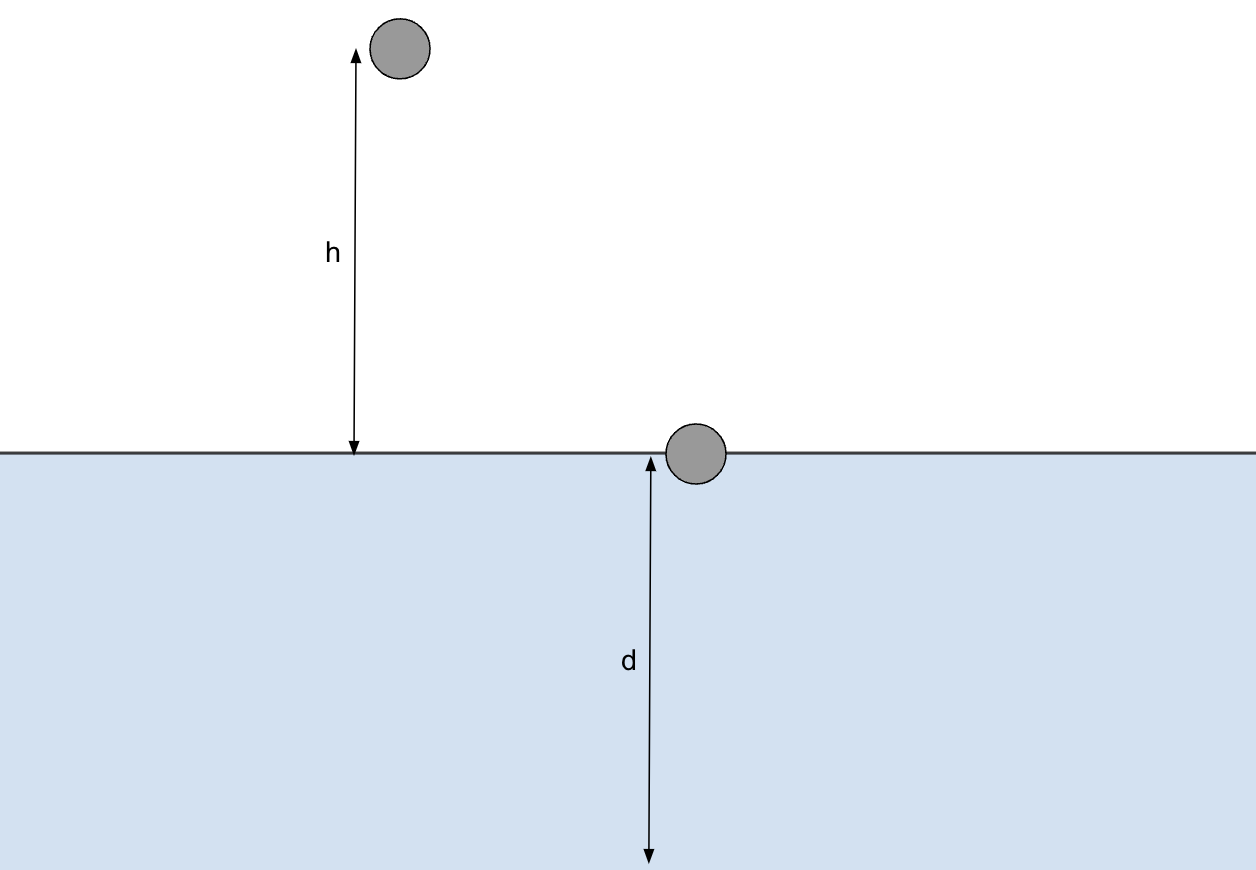
\includegraphics[scale=0.42]{problems/figures/ballDiagram.png}
% \end{figure}
% \FloatBarrier
\end{problem}